%\documentclass[12pt,letterpaper]{article}\usepackage{epsfig,amsmath,amssymb,natbib,ifthen,hyperref}\provideboolean{StandAlone}\setboolean{StandAlone}{true} \begin{document}
%\documentclass[12pt,letterpaper]{article}\usepackage{epsfig,float,amsmath,dcolumn,multicol,latexsym,ifthen,natbib,amssymb,verbatim,hyperref,vmargin,moreverb,cancel,psibycus}\def\mathkoppa{\text{\koppa}}\newcommand{\koppa}{{\greek{}k+}}\newcommand{\Koppa}{{\greek{}K+}}\provideboolean{StandAlone}\setboolean{StandAlone}{true} \begin{document}

The above discussion suggested that precautionary behavior can be understood by considering a tradeoff between
the present (captured by $u(c_{t})$) and the future (captured by ${\omega}_{t}({m}_{t}-{c}_{t})$).

That analysis was incomplete in a crucial respect: It took the initial
level of resources, ${m}_{t}$, as given exogenously.  But arguably the
most important question about precautionary behavior is how large an
effect it has on the prevailing level of ${m}$. This cannot be
answered using a framework that treats ${m}$ as exogenous.

The framework can be extended to address this problem, by defining the
problem in such a way that the functions $v$ and ${\omega}$ reflect
the discounted value of an infinite number of future periods.  This is
often accomplished by making assumptions under which optimal behavior
in every future period is identical to optimal behavior in the current
period; it is then possible to solve for a ``consumption function''
that provides a complete characterization of the relationship between
resources and spending.

The critical extra assumption is ``impatience,'' broadly construed as a condition
on preferences that prevents wealth (or the wealth to income ratio) from growing to infinity.  In the simplest version
of the model where income does not grow, the required condition is
$R\beta < 1$; for the appropriate condition in models with income growth,
see~\cite{BufferStockTheory}.

The exact nature of income risk turns out to be less important than
the assumption of impatience.  Here, we analyze a particularly simple
case (which is an adaptation of a model by \cite{toche:urisk}).  There
are two kinds of consumers: workers and retirees.  Retirees have no
labor income, and must live off their assets.  Workers earn a fixed
amount of labor income in each period, but face a constant danger of
being exogenously forced into retirement. (Exogenous forced retirement
is the sole source of risk in the model).

Under these assumptions, if the utility function is of the standard constant relative risk aversion form
$u(c)=c^{1-\rho}/(1-\rho)$, optimal behavior for retirees is very simple: They spend a constant
fraction of ${m}$ in each period, where the fraction depends on the degree of impatience and 
intertemporal substitution $(1/\rho)$.

The situation for workers is more interesting; it is depicted in
figure~\ref{fig:ConsFunc}.

The simplest element of the figure is the line labelled ``Perm Inc.'' This shows, for any ${m}$, the
level of spending that would leave expected ${m}$ unchanged; it is equal to labor income plus the interest on
capital income, and is upward sloping because a consumer with more ${m}$ earns more capital income.

The assumption of impatience is reflected in the fact that the
consumption function that would apply if uncertainty did not exist,
$\bar{c}({m})$, is everywhere above the level of permanent income
(income of the perfect-certainty consumer is adjusted downward so that
the reduction in unemployment risk does not cause an increase in mean
income).  In other words, an impatient consumer facing no uncertainty
would choose to spend at a rate that cannot be sustained indefinitely.

The locus with arrows is the consumption function, which indicates the
optimal level of spending (in the presence of uncertainty) for any
given level of ${m}$.  Since the difference between ${c}({m})$ and
$\bar{c}({m})$ is purely the consequence of risk, that difference
$\bar{c}({m})-{c}({m})$ constitutes the amount of precautionary saving
associated with any specific ${m}$.

Standard assumptions about preferences and uncertainty imply that
there will be an intersection between the permanent income locus and
the consumption function.  (For a proof that there will be only one
intersection, see~\cite{BufferStockTheory}).  The intersection defines
a ``target'' level for the buffer stock of wealth ${m}$: The level such that an employed consumer
with this amount of resources today will end up with the same $m$ next period.  
Dynamics are captured by the
arrows, which indicate that, for initial
values of ${m}$ below the target, consumption is below permanent
income, so $m$ is increasing and consumption crawls upward along the
consumption function toward the target.  For initial values of
${m}$ above the target, consumption is above permanent income, so $m$
is falling.  The consumer holds a ``buffer stock'' of wealth in an attempt
to reach the ``target'' level of wealth as defined above.  

The existence of a target level of resources has many interesting
implications.  Perhaps the most surprising is that in long-run equilibrium the
expected growth rate of consumption for employed consumers is
unrelated to the interest rate or the degree of impatience.

To understand this point better, and to relate it to the literature,
we restate it in a slightly more general form:  The equilibrium
expected growth rate of consumption for employed consumers is
approximately equal to their predictable rate of income growth,
\begin{eqnarray}
  \label{eq:CGrow}
  \mathbf{E}_{t}[\Delta \log {c}_{t+1}^{e}] & \approx & g.
\end{eqnarray}

In many respects the equilibrium equality of consumption growth and
permanent income growth seems intuitive. However, it
appears to conflict with a standard way of analyzing consumption
growth, which relies on the first order condition from the
optimization problem (the `Euler equation'), which is often
approximated by an equation of the form
\begin{eqnarray}
  \label{eq:CGrowPF}
  \mathbf{E}_{t}[\Delta \log {c}^{e}_{t+1}] & \approx & \rho^{-1}(r-\tau) + \phi
\end{eqnarray}
where $\rho$ is the coefficient of relative risk aversion and $\tau$
is the geometric rate at which future utility is discounted (related
to the time preference factor $\beta$); $\phi$ is a term that
reflects the contribution of precautionary motives to consumption
growth.

The resolution of the apparent contradiction is that the precautionary
component of consumption growth is endogenous; combining
\eqref{eq:CGrow} and \eqref{eq:CGrowPF} permits us to solve for the
equilibrium value of the precautionary contribution to consumption
growth:
\begin{eqnarray}
  \label{eq:phi}
  \phi & \approx & g - \rho^{-1}(r-\tau).
\end{eqnarray}

We return to this point below.

% Impatience vs prudence

%\subsection{Concavity of the Consumption Function}

We can characterize the effect of uncertainty by noting three facts
about figure~\ref{fig:ConsFunc}: $c({m}) < \bar{c}({m})$ (consumption is lower in the presence of uncertainty);
$\lim_{{m} \rightarrow \infty} \bar{c}({m})-c({m}) = 0$  (as wealth
approaches infinity the effect of uncertainty in labor income vanishes); and
$c({m})$ is strictly concave, so that the marginal propensity to consume
out of a windfall increase in income, $c^{\prime}({m}),$ is greater for
poor people than for rich people.

The concavity of the consumption function bears further comment.
Intuitively, it can be understood in a similar light to the effect of
liquidity constraints. A consumer who is subject to a
currently-binding liquidity constraint is someone for whom a marginal
increase in cash will result in an immediate one-for-one increase in
spending (a marginal propensity to consume (MPC) of one).  However, if
the same consumer happened to have a large windfall transfer of cash
(say, he wins the lottery), he would no longer be currently
constrained, and his MPC would (presumably) be less than one.  In the
case of precautionary saving, the ownership of an extra unit of wealth
relaxes the suppression of consumption due to risk; this relaxation is
more powerful for low-wealth consumers living on the edge of
(precautionary) fear than for high wealth consumers with plenty of
resources.  Thus, either liquidity constraints or precautionary
motives or both will cause the consumption function to become concave
(\cite{carroll&kimball:liquidity}). \cite{huggett:higherW} shows that
consumption concavity in turn implies greater equilibrium wealth.  

Empirical evidence indicates that the wealth distribution is highly
concentrated.  This means that the owners of much of the aggregate
capital stock likely inhabit the portion of the consumption function
to the far right, where it approaches the linear consumption function
that characterizes the perfect foresight solution.  Note, however,
that this does not necessarily imply that aggregate consumption
behavior will resemble that of a perfect foresight consumer, because a
large proportion of aggregate consumption is accounted for by
households with small amounts of market wealth.  Spending of such
households is likely determined much more by their permanent income
than by their meager wealth, and so it remains possible that a high
proportion of consumption is performed by households inhabiting the
more nonlinear part of the consumption function.

\begin{figure}[ht]
\caption{The Consumption Function}
\centerline{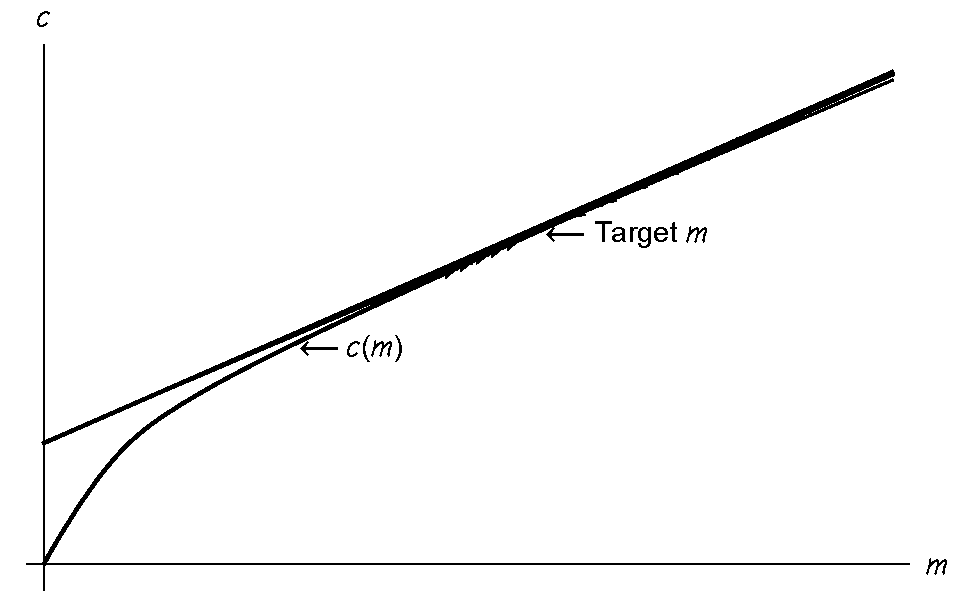
\includegraphics[width=5.5in]{./Figures/PalgraveTargetPlot}}
\label{fig:ConsFunc}
\end{figure}

\ifthenelse{\boolean{StandAlone}}{\end{document}}{}
